%Jennifer Pan, August 2011

\documentclass[10pt,letter]{article}
	% basic article document class
	% use percent signs to make comments to yourself -- they will not show up.
\usepackage{enumerate}
\usepackage{amsmath}
\usepackage{amssymb}
	% packages that allow mathematical formatting

\usepackage{graphicx}
	% package that allows you to include graphics

\usepackage{setspace}
	% package that allows you to change spacing

\onehalfspacing
	% text become 1.5 spaced

\usepackage{fullpage}
	% package that specifies normal margins
	

\begin{document}
	% line of code telling latex that your document is beginning


\title{Homework 1}

\author{SABIC: Physics}

\date{Due January 21, 2016}
	% Note: when you omit this command, the current dateis automatically included
 
\maketitle 
	% tells latex to follow your header (e.g., title, author) commands.

\section*{Reading (Due April 1, 2015):}
Read Chapter 1.
\section*{Problem 1: practice with estimation}
\begin{enumerate}[(a)]
\item How many kernels of corn does it take to fill a 2 liter soda bottle?
\item How many liters of gasoline are used in the United States in one day? 
\end{enumerate}
\section*{Problem 2: conceptual}
\begin{enumerate}[(a)]
\item What physical phenomena could you use to define a time standard?
\item Describe how you could measure the thickness of a sheet of
paper with an ordinary ruler.
\item Can you find two vectors with different lengths that have a
vector sum of zero? What length restrictions are required for three
vectors to have a vector sum of zero? Explain your reasoning.
\item(i) Does it make sense to say that a vector is negative?
Why? (ii) Does it make sense to say that one vector is the negative
of another? Why? Does your answer here contradict what you said
in part (i)?
\item 
\end{enumerate}
\section*{Problem 3: vector addition}
\begin{figure}[!ht]
  \centering
    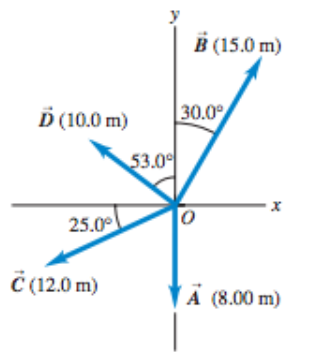
\includegraphics[width=0.5\textwidth]{fig1.png}
\end{figure}
\begin{enumerate}[(a)]
\item For the vectors $\vec{A}$ and $\vec{B} $in the figure, find the magnitude and direction of (i) $\vec{A} + \vec{B}$, (ii) $\vec{A} - \vec{B}$, (iii) $-\vec{A} - \vec{B}$, and (iv) $\vec{B} - \vec{A}$.
\item A spelunker is surveying a cave. She follows a passage 180 m straight west, then 210 m in a direction $45^\circ$ east of south, and then 280 m at $30^\circ$ east of north. After a fourth unmeasured displacement, she finds herself back where she started. Use a scale drawing to determine the magnitude and direction of the fourth displacement. 
\end{enumerate}
\section*{Problem 4: vector multiplication}
\begin{enumerate}[(a)]
\item For the vectors $\vec{A}$, $\vec{B}$, and $\vec{C}$ in the figure, find $\vec{A}\cdot\vec{B}$, $\vec{A}\cdot\vec{C}$, and $\vec{B}\cdot\vec{C}$.
\item For the vectors $\vec{A}$ and $\vec{D}$ in the figure, find the magnitude and direction of $\vec{A} \times \vec{D}$ and $\vec{D} \times \vec{A}$.
\end{enumerate}

\end{document}
	% line of code telling latex that your document is ending. If you leave this out, you'll get an error
